\chapter{Case Study and Data Engineering}
\label{chp:case_study_and_data}

This chapter describes the operational context and the pipeline that turns raw operational
records into a simulation-ready event log. The resulting event log is the input for Chapters~\ref{chp:experiments} and~\ref{chap:results}.

Section~\ref{sec:cs_environment} introduces HHLA Container Terminal
Burchardkai (CTB), the truck-handling operations and the data sources.
Section~\ref{sec:event_log_engineering} describes how the pipeline reconstructs lifecycle timestamps and derives the case-level context required by ProSiT
\cite{Vinci2026prosit}. The final section describes the event log and its
characteristics used for the temporal train/validation/test split in
Section~\ref{sec:train_test_split}.

The Truck schedule serves as the baseline for the data assembly.

In a first step, the raw schedule is cleaned from false or incomplete entries. That includes missing timestamps and total visit times of over 12 hours, as those indicate system errors. 

We are matching container details to each recorded transatction to give each visit with its operations complexity.
Using ProSiT as the simulation framework in this thesis, we are then aggregating the individual container details to a case level complexity. Container attributes, like dangerous goods, fill status etc. are transformed into a complexity code system attributing each visit with a complexity score and container counts and trafic direction. 

Then the schedules attributes and timestamps are transformed into an event log style.  
Then the system variables are added by the initial timestamp of the process, aka the moment, the truck enters the terminal. 
The demand of the gate at moment of entry, as well as the demand at the planned transaction points are calculated. 

To include the terminals utilization into the process behaviour, the utilization of each of the yard sections and blocks is calculated and added to each visit. 

[INCLUDE TARGET FEATURES? SO FILTER OUT DOUBLE BLOCK VISITS?]




%%%%%%%%%%%%%%%%%%%%%%%%%%%%%%%%%%%%%%%%%%%%%%%%%%%%%%%%%%%%%%
\section{Case Study Environment}
\label{sec:cs_environment}
%%%%%%%%%%%%%%%%%%%%%%%%%%%%%%%%%%%%%%%%%%%%%%%%%%%%%%%%%%%%%%

    \subsection{HHLA Container Terminal Burchardkai}

    This case study concerns the HHLA Container Terminal Burchardkai (CTB) in the Port of Hamburg. CTB handles approximately 2.6 million TEU
    (Twenty-foot Equivalent Units) annually across 315 hectares
    \cite{hhla2025}.

    \textbf{Truck process.} External trucks visit CTB to deliver or receive
    containers. At \textit{Gate In}, the truck is registered at the entry
    gate. It then drives to the assigned yard position, where an RMG or other
    handling equipment loads or unloads the container. After all planned
    operations are completed, the truck leaves through \textit{Gate Out}.

    The CTB environment in this project has several resource constraints.
    Located between the waterside and the landside, 22 RMG storage
    blocks (T06--T27) serve both sides. Operational experts from the terminal
    confirmed two constraints used in this study: the activities of one truck
    cannot be executed in parallel, and at most three automated rail-mounted
    gantry cranes can work concurrently at one block. The CTB
    has two specialised areas: an empty-container depot (called
    ``MT'' or ``LL'', from the German \textit{Leerlager}) and the
    manually operated HO2 yard area. The terminal gate consists of 16
    lanes, split between incoming and outgoing trucks. The number of
    operated gate lanes varies by day, shift and terminal resource plan.

    \subsection{Data Sources}
    \label{sec:cs_data_sources}

    The data come from several systems used in daily terminal operations.
    These systems were developed over time and record different parts of the
    process. A Terminal Operating System coordinates them.
    Table~\ref{tab:ctb_data_sources} summarises the four sources used in this
    thesis.

\begin{table}[htbp]
\centering
\begin{tabularx}{\textwidth}{L{4.4cm}Y}
\toprule
\textbf{Data source} & \textbf{Data provided} \\
\midrule
ITS schedule & Truck-visit schedules and timestamps for gate entry,
handling readiness, order completion and gate exit. \\
Report system & Stage-level execution data, gate-entry records,
exchange-area assignments, container transactions and carrier identifiers. \\
Yard management system & Four-hour snapshots of storage-block capacity,
occupancy and utilisation. \\
Container master data & Container size, type, loading status, hazardous and
reefer indicators, dwell time and inbound/outbound carriers. \\
\bottomrule
\end{tabularx}
\caption{Operational data sources used for event-log engineering.}
\label{tab:ctb_data_sources}
\end{table}

    These systems generate independent data pools with different
    identifier schemes, requiring a data-integration procedure
    described in Section~\ref{sec:event_log_engineering}. Historical
    data from March and April 2026 (approximately eight weeks) were extracted.
    The raw extract covers approximately 104,000 truck visits, 113,466
    container move events and 336 yard-state snapshots
    ($8$ weeks $\times 7$ days $\times 6$ snapshots per day).
    The move-event count refers to the raw report-system extract. It is not the
    denominator used later for the cleaned and cross-system-matched schedule
    records.

%%%%%%%%%%%%%%%%%%%%%%%%%%%%%%%%%%%%%%%%%%%%%%%%%%%%%%%%%%%%
\section {Case Construction}
\textit{
\begin{enumerate}
    \item Data Sources
    \item Visit reconstruction by Keys, Assumptions, Containers, 
    \item Timestamp Semantics
    \item Ressource Identities
    \item Cleaning
    \item Data Split
\end{enumerate}
}
\FloatBarrier

\subsection{Context Enrichment}
\label{sec:context_enrichment}

To enable data-aware simulation, the event log is enriched with
contextual attributes describing the operational state at the time of
process execution. These attributes are organised into five
categories.

\paragraph{Information Available at Truck Entry}
\label{sec:entry_known_attributes}

The scheduling record contains the complete planned visit manifest before
the truck enters the terminal. The number of planned stops,
the numbers of delivery and receive transactions, the planned target area
and the resulting final visit-complexity score are known at Gate In. The
pipeline reproduces this entry-time information by aggregating all rows of
the same \texttt{FAHRPLAN\_UID}. It does not infer these attributes from
later realised durations or completion outcomes.
\texttt{visit\_complexity} is a deterministic summary of the planned
stop/container manifest (visit size, container-handling complexity and
mixed-flow complexity), not an ex-post performance measure. Using these
variables as case attributes does not leak the simulated future
provided that the same planned manifest is supplied for a prospective run.

The implementation detail that the target block is reconstructed from the
planned stop's area-specific activity label can otherwise look like
look-ahead: after genericising \texttt{T06--T27} activities, the reconstructed
block is copied into \texttt{primary\_target\_area}. Semantically, however,
the source is the planned \texttt{ANLAUFPUNKT\_HALTESTELLE} attached to the
visit order and available at entry, not the later activity-completion
timestamp. This distinction defines the deployment contract for all
entry-known case attributes.

\paragraph{Container Features}

Container-related context is aggregated to case level so that visit
properties can serve as case-level attributes in ProSiT. The resulting
\texttt{n\_containers} attribute counts the unique containers handled during
the visit. The binary attributes \texttt{has\_hazardous} and
\texttt{has\_reefer} are aggregated using a logical OR across the complete
manifest. The \texttt{full\_ratio} records the share of loaded containers,
while \texttt{container\_complexity\_mean} and
\texttt{container\_complexity\_sum} describe the average and cumulative
handling complexity of the visit.

\paragraph{Yard Features}

Yard state features capture the storage capacity and utilisation status
of different terminal areas at truck arrival (Gate In event). These
features are matched by an exact equality join on the minute-resolved Gate In
timestamp. The joined snapshot provides the overall
\texttt{gate\_utilization}, the aggregated \texttt{rmg\_utilization}, and
the area-level \texttt{vc\_utilization} and \texttt{mt\_utilization}. For
single-block visits, \texttt{target\_utilization} gives the utilisation of
the assigned RMG block.

\paragraph{Demand Features}

Demand features quantify operational load pressure at different
terminal areas over a rolling 60-minute window. The general
\texttt{gate\_demand} counts trucks processed across the terminal during the
preceding hour. The \texttt{rmg\_demand}, \texttt{vc\_demand} and
\texttt{mt\_demand} attributes separate this load by operational area.
For single-block visits, \texttt{target\_demand} records the demand for the
assigned RMG block.


%%%%%%%%%%%%%%%%%%%%%%%%%%%%%%%%%%%%%%%%%%%%%%%%%%%%%%%%%%%%%%
\section{Observed Truck-Visit Behaviour}
\label{sec:observed_behaviour}
%%%%%%%%%%%%%%%%%%%%%%%%%%%%%%%%%%%%%%%%%%%%%%%%%%%%%%%%%%%%%%
% Source: trucksimulation/peak_analysis/peak_analysis_observed_v2.py,
% output peak_analysis/observed_20261007_v2. Training and validation only.

This section describes the recorded behaviour that the simulation must
reproduce. It covers the visit structure, the arrival pattern, the
turnaround time and the conditions under which delays occur. All
statements are descriptive associations. They do not establish causes.
Thresholds are fitted on the training partition and applied unchanged
to the validation partition. The test partition is not used.

\subsection{Visit Structure and Turnaround Time}
\label{sec:obs_structure}

Table~\ref{tab:obs_descriptives} summarises both partitions. Nine out of
ten visits have a single yard stop. Visits with three or more stops are
rare. Receive and delivery visits are similarly frequent, and about one
visit in seven is mixed. About a quarter of the visits do not use an RMG
block. Visits with two different RMG blocks make up 1.7\,\% of the
training visits.

\begin{table}[htbp]
\centering
\begin{tabularx}{\textwidth}{YL{2.6cm}L{2.6cm}}
\toprule
\textbf{Measure} & \textbf{Training} & \textbf{Validation} \\
\midrule
Visits & 58,262 & 14,625 \\
Visits with 1 / 2 / $\geq$3 stops & 91.3 / 8.6 / 0.2\,\% & 89.8 / 10.1 / 0.1\,\% \\
Delivery / receive / mixed visits & 38.6 / 48.2 / 13.2\,\% & 42.2 / 43.4 / 14.5\,\% \\
No RMG / one block / several blocks & 22.5 / 75.7 / 1.7\,\% & 27.1 / 70.8 / 2.1\,\% \\
\midrule
TTT mean / median / P90 [min] & 36.5 / 28.5 / 64 & 42.2 / 34 / 78 \\
Median TTT delivery / receive / mixed & 23 / 30 / 41 & 28 / 35 / 48 \\
Median TTT one block / several blocks & 29 / 46.5 & 33 / 50 \\
Mean approach / stops / transfer / exit & 10.9 / 12.0 / 1.1 / 12.5 & 13.2 / 13.7 / 1.5 / 13.6 \\
\bottomrule
\end{tabularx}
\caption{Visit structure and turnaround time (TTT) by partition. Approach
is the time from Gate In to the start of the first stop, exit the time
from the end of the last stop to Gate Out, and transfer the time between
stops. Because gate events are instantaneous, the four components add up
to the TTT.}
\label{tab:obs_descriptives}
\end{table}

The turnaround time depends on the type of visit. Receive visits take
longer than delivery visits, and mixed visits take longest. A visit with
two RMG blocks takes about 17 minutes longer than a single-block visit.
The decomposition shows that the stop intervals account for only about
one third of the mean TTT. Approach and exit together account for about
two thirds. Since a stop interval begins when the truck reports ready in
the handover lane, it can already contain waiting for the crane. Driving
and any queueing before the truck reports ready fall into the approach.

\subsection{Arrival Pattern}
\label{sec:obs_arrivals}

Trucks arrive in a stable weekly and daily pattern
(Figure~\ref{fig:obs_calendar}). Arrivals take place from Monday to
Friday, with few visits on Saturdays and none on Sundays. On weekdays,
about 22 trucks per hour arrive between midnight and 5:00. The rate
rises to about 118 per hour at 6:00 and stays on a plateau of 126 to 152
trucks per hour between 7:00 and 16:00. After 17:00 it falls again. The
week around Easter (1 to 7 April) has a markedly lower volume.

An \emph{arrival peak} is a Gate-In hour with at least 165 arrivals, the
90th percentile of all training hours with arrivals. Arrival peaks are
short spikes on top of the daytime plateau. They make up 70 of 610
training hours with at least 20 visits (11.5\,\%) and 18 of 147
validation hours. The highest hourly count is 255 trucks, in the
validation period.

\begin{figure}[htbp]
\centering
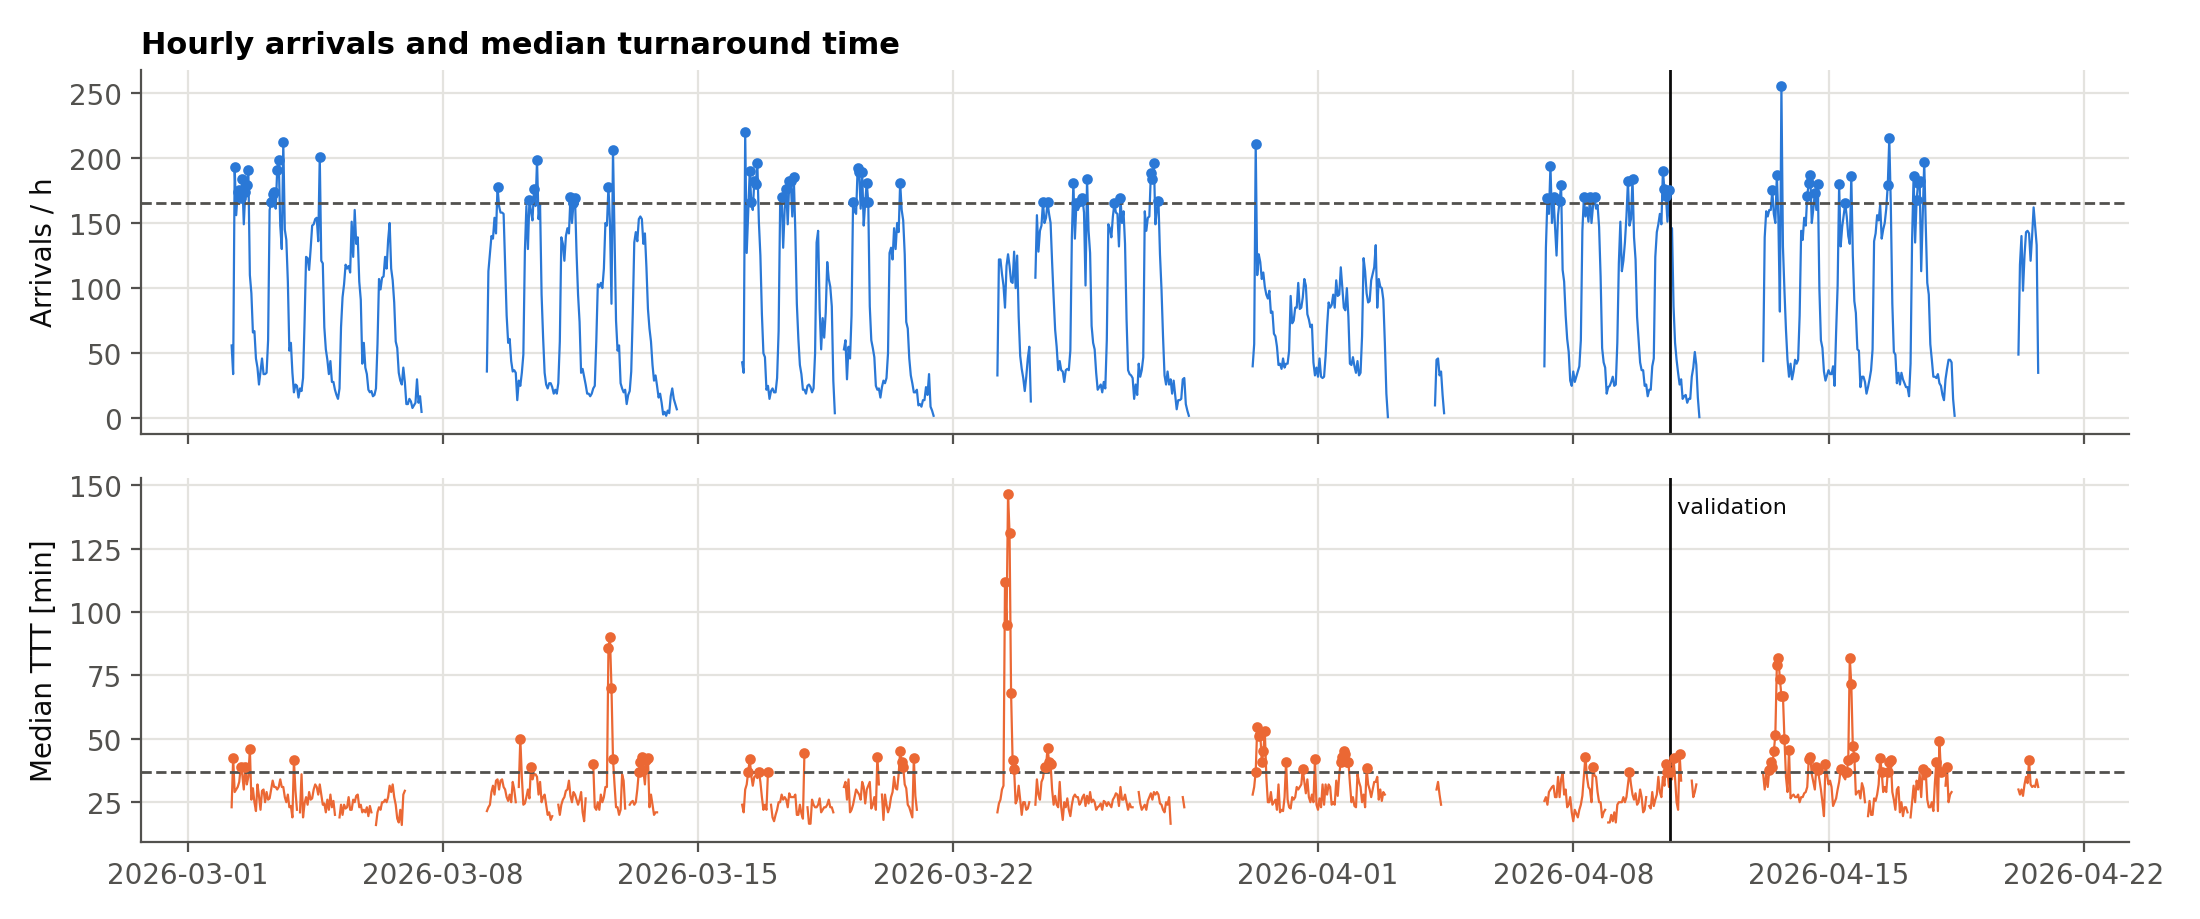
\includegraphics[width=\textwidth]{figures/observed/hourly_arrivals_ttt.png}
\caption{Hourly arrivals (top) and median turnaround time by Gate-In hour
(bottom) for the training and validation periods. Dots mark arrival peaks
and delay peaks. Dashed lines show the thresholds of 165 arrivals and
37 minutes. The vertical line marks the start of the validation period.}
\label{fig:obs_calendar}
\end{figure}

\subsection{Congestion over the Day}
\label{sec:obs_congestion}

The turnaround time grows over the working day, although the arrival
rate stays on its plateau. On training weekdays, the median TTT rises
from 26 minutes for trucks arriving at 7:00 to 34 minutes at 14:00. The
P90 rises from 57 to 81 minutes at 13:00. The mean number of trucks
already inside the terminal at Gate In grows from 69 at 7:00 to 106 at
15:00. Figure~\ref{fig:obs_components} shows that this growth comes mainly
from the approach and the exit. The stop intervals change comparatively
little over the day.

\begin{figure}[htbp]
\centering
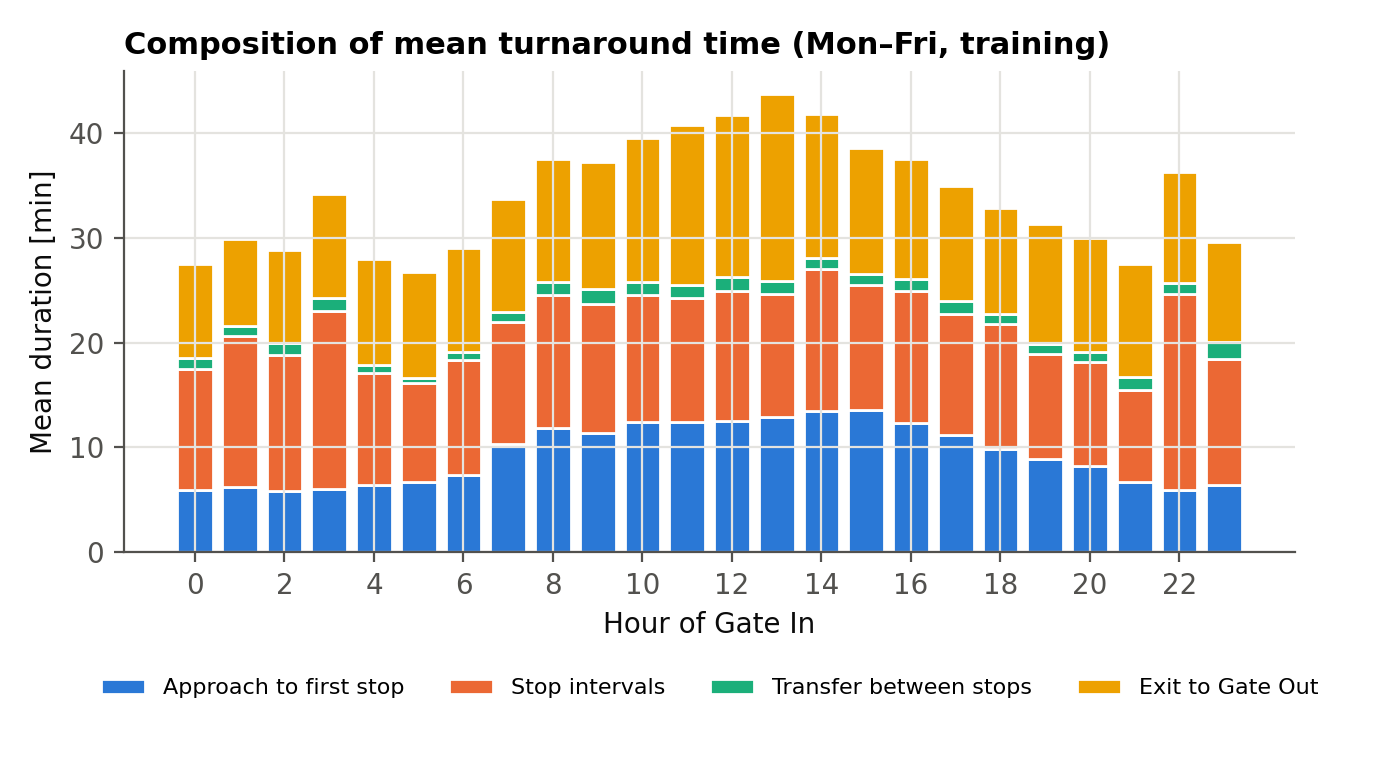
\includegraphics[width=0.85\textwidth]{figures/observed/ttt_components_by_hour.png}
\caption{Mean turnaround time by Gate-In hour, split into approach, stop
intervals, transfer and exit. Training weekdays.}
\label{fig:obs_components}
\end{figure}

The turnaround time increases with the number of trucks in the terminal,
and the increase is non-linear (Figure~\ref{fig:obs_wip}). Up to about
100 trucks, the median TTT rises slowly from 23 to 34 minutes. Between
140 and 160 trucks, the median reaches 43 minutes and the P90 about 100
minutes. Above 160 trucks, the P90 exceeds two hours. Such occupancy
levels are rare and occur on a few days only. The
Spearman correlation between hourly arrivals and the median TTT of the
same hour is 0.51. It is 0.53 for the arrivals of the preceding three
hours and drops to 0.05 for a lag of six hours.

\begin{figure}[htbp]
\centering
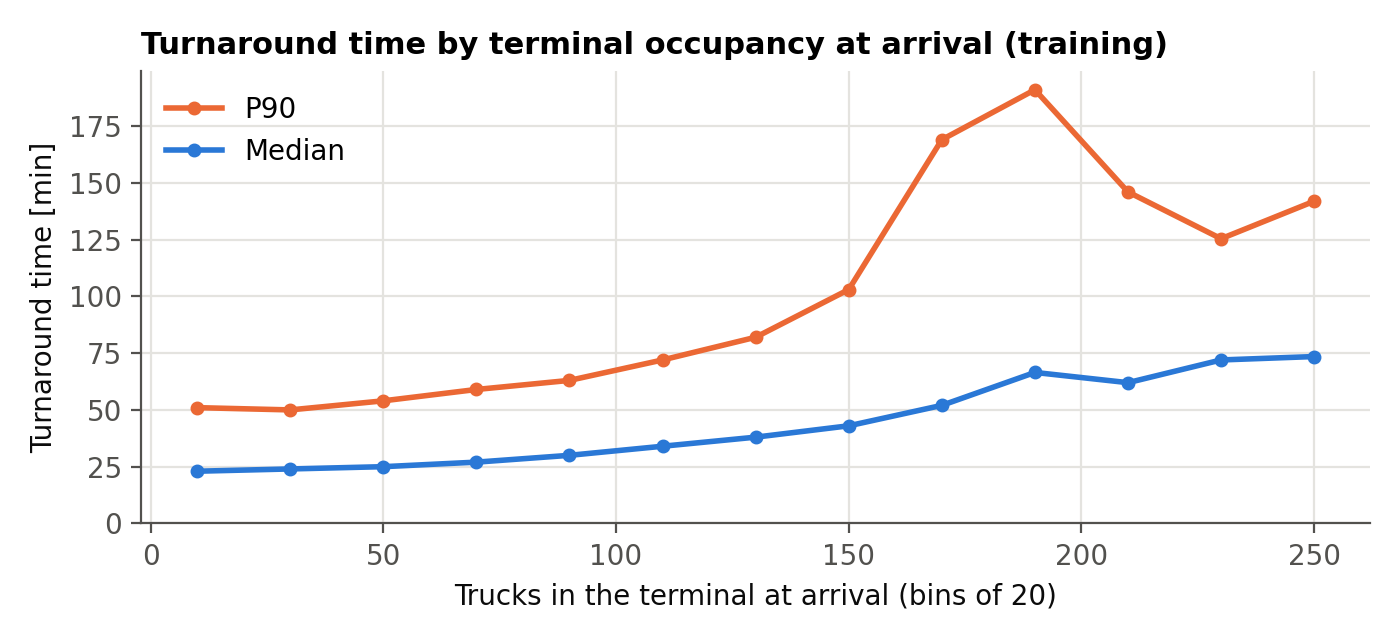
\includegraphics[width=0.85\textwidth]{figures/observed/ttt_vs_wip.png}
\caption{Median and P90 of the turnaround time by the number of trucks
in the terminal at Gate In, in classes of 20. Training, classes with at
least 50 visits.}
\label{fig:obs_wip}
\end{figure}

The same pattern appears at the handling units
(Figure~\ref{fig:obs_unit}). At an RMG block, the median stop interval
is 5 minutes when the truck is alone at the block. It is 9, 13 and 18
minutes when two, three or four trucks have an open interval at the same
block. The Spearman correlation between unit occupancy and stop duration
is 0.49 for RMG, 0.45 for LL and 0.32 for HO2. Up to four concurrent
intervals occur at an RMG block, although a block has three handover
lanes. How a fourth interval arises is not yet clear. At LL and HO2,
more than ten concurrent intervals occur. This confirms that the
timestamps of these areas do not represent physical occupancy.

\begin{figure}[htbp]
\centering
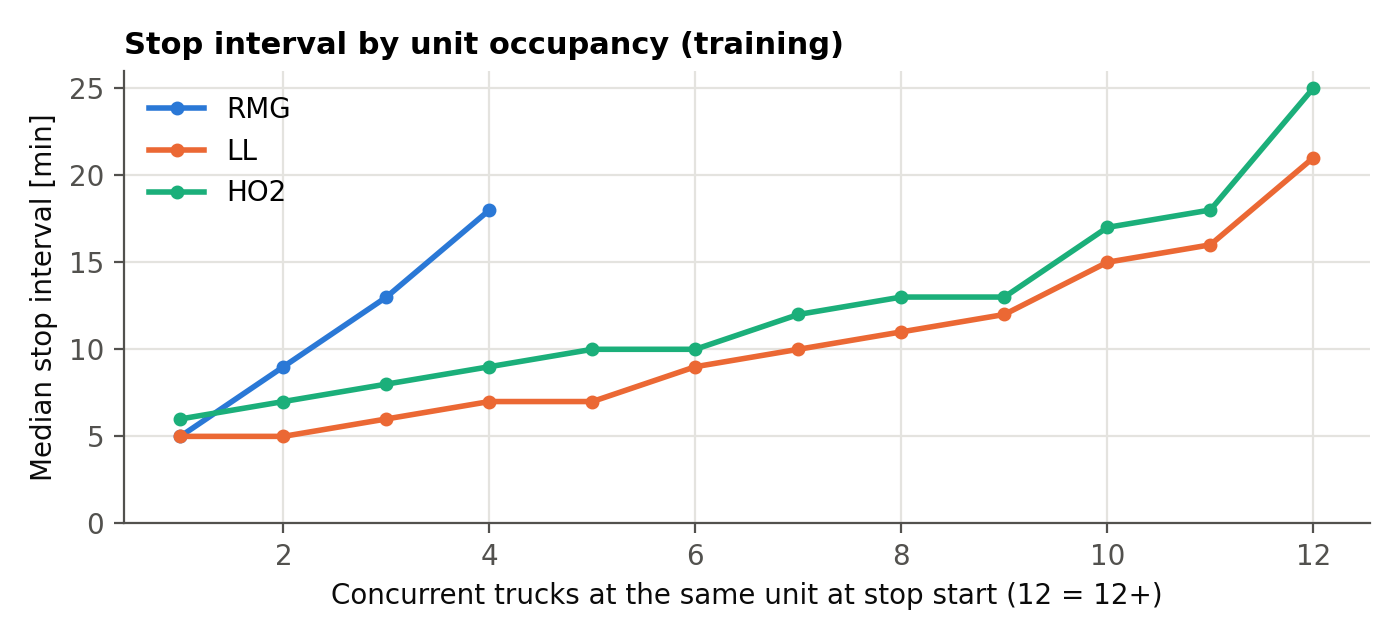
\includegraphics[width=0.85\textwidth]{figures/observed/stop_vs_unit_wip.png}
\caption{Median stop interval by the number of trucks with an open
interval at the same handling unit when the stop starts. Training.}
\label{fig:obs_unit}
\end{figure}

\subsection{Delay Peaks}
\label{sec:obs_delay_peaks}

A \emph{delay peak} is a Gate-In hour with at least 20 visits whose
median TTT is at least 37 minutes, the 90th percentile of the training
hours. Delay peaks are a different phenomenon from arrival peaks.
Training contains 62 delay-peak hours (10.2\,\%) and validation 39
(26.5\,\%). Only nine delay-peak hours in each partition are also
arrival-peak hours.

Table~\ref{tab:obs_peak_components} decomposes the turnaround time in
and outside delay peaks. In training, the mean TTT in delay-peak hours
is 24.4 minutes longer. Approach and exit account for 21.4 minutes of
this difference, or 88\,\%. The stop intervals grow by only 2.5 minutes.
Arrival peaks, in contrast, are associated with an increase of only 2.4
minutes in mean TTT.

\begin{table}[htbp]
\centering
\begin{tabularx}{\textwidth}{YL{1.5cm}L{1.5cm}L{1.5cm}L{1.5cm}L{1.5cm}}
\toprule
\textbf{Training, mean [min]} & \textbf{Approach} & \textbf{Stops} & \textbf{Transfer} & \textbf{Exit} & \textbf{TTT} \\
\midrule
Delay-peak hours (7,273 visits) & 19.3 & 14.2 & 1.6 & 22.9 & 57.9 \\
Other hours (50,989 visits) & 9.8 & 11.7 & 1.1 & 11.0 & 33.5 \\
Difference & +9.5 & +2.5 & +0.5 & +11.9 & +24.4 \\
\midrule
Arrival-peak hours (12,732 visits) & 12.0 & 12.4 & 1.2 & 12.9 & 38.4 \\
Other hours (45,530 visits) & 10.7 & 11.9 & 1.1 & 12.3 & 36.0 \\
\bottomrule
\end{tabularx}
\caption{Turnaround-time components in and outside peak hours. Visits
are assigned to the hour of their Gate In.}
\label{tab:obs_peak_components}
\end{table}

Not all visits are affected equally. In arrival peaks, the median TTT of
receive visits rises from 28 to 34 minutes, that of delivery visits only
from 23 to 25 minutes. Multiblock visits rise from 45 to 52 minutes.
Visits without RMG are almost unaffected (27 to 28 minutes). Among the
RMG blocks, T18 shows the largest increase of the median stop interval,
from 10 to 17 minutes. Most other blocks increase by at most three
minutes, and HO2 stops are not longer in arrival peaks.

\subsection{Disruption Episodes}
\label{sec:obs_episodes}

A few delay peaks follow a different pattern. On Monday, 23 March 2026,
the hourly median TTT rose to between 112 and 146 minutes from about
9:30, while arrivals stayed at a normal 85 to 126 trucks per hour. Up to
306 trucks were inside the terminal. The additional time lies almost
entirely in the exit, with approach and stop intervals at normal values.
Similar but shorter episodes occur on 12 March and on 13 April
(validation). Possible explanations include a disruption at the exit
gate or in exit processing, or an artefact of the Gate Out recording.
% TODO: add the explanation from the domain review (questionnaire D9).
Such episodes are not driven by demand. A simulation learned from normal
operations cannot be expected to reproduce them. They are therefore
identified by a rule fixed in advance and reported separately, but they
are never removed from the evaluation.

\subsection{Differences between the Partitions}
\label{sec:obs_drift}

The validation period is more congested than the training period. Its
daily median TTT is 32 minutes against 29, and the share of delay-peak
hours is 26.5\,\% against 10.2\,\%. Visits without RMG show the largest
shift, with a median TTT of 39 against 27 minutes. A model fitted on the
training period is therefore expected to underestimate the validation
TTT, independently of its control flow. For this reason, model variants
are compared with each other on the same period, and absolute
deviations are interpreted with this shift in mind.

\subsection{Implications for the Simulation}
\label{sec:obs_implications}

The observed behaviour defines what an adequate simulation must
reproduce for the purpose of this thesis.

\begin{enumerate}
\item The weekday and hourly arrival profile, including arrival peaks
above 165 trucks per hour.
\item The stop structure and the turnaround time by visit type.
\item The increase of the turnaround time with the number of trucks in
the terminal, and of the stop interval with the occupancy of the unit.
\item The growth of approach and exit time under load, since these
components carry most of the delay in delay-peak hours.
\item Delay peaks at a frequency comparable to the observed one,
excluding disruption episodes, which are reported separately.
\end{enumerate}

These requirements are the basis of the comparison measures in
Chapter~\ref{chp:experiments}.

\section{Domain Rules}
\textit{Documenting the origin of Domain Rules and operational requirements}

